\documentclass[1p]{elsarticle_modified}
%\bibliographystyle{elsarticle-num}

%\usepackage[colorlinks]{hyperref}
%\usepackage{abbrmath_seonhwa} %\Abb, \Ascr, \Acal ,\Abf, \Afrak
\usepackage{amsfonts}
\usepackage{amssymb}
\usepackage{amsmath}
\usepackage{amsthm}
\usepackage{scalefnt}
\usepackage{amsbsy}
\usepackage{kotex}
\usepackage{caption}
\usepackage{subfig}
\usepackage{color}
\usepackage{graphicx}
\usepackage{xcolor} %% white, black, red, green, blue, cyan, magenta, yellow
\usepackage{float}
\usepackage{setspace}
\usepackage{hyperref}

\usepackage{tikz}
\usetikzlibrary{arrows}

\usepackage{multirow}
\usepackage{array} % fixed length table
\usepackage{hhline}

%%%%%%%%%%%%%%%%%%%%%
\makeatletter
\renewcommand*\env@matrix[1][\arraystretch]{%
	\edef\arraystretch{#1}%
	\hskip -\arraycolsep
	\let\@ifnextchar\new@ifnextchar
	\array{*\c@MaxMatrixCols c}}
\makeatother %https://tex.stackexchange.com/questions/14071/how-can-i-increase-the-line-spacing-in-a-matrix
%%%%%%%%%%%%%%%

\usepackage[normalem]{ulem}

\newcommand{\msout}[1]{\ifmmode\text{\sout{\ensuremath{#1}}}\else\sout{#1}\fi}
%SOURCE: \msout is \stkout macro in https://tex.stackexchange.com/questions/20609/strikeout-in-math-mode

\newcommand{\cancel}[1]{
	\ifmmode
	{\color{red}\msout{#1}}
	\else
	{\color{red}\sout{#1}}
	\fi
}

\newcommand{\add}[1]{
	{\color{blue}\uwave{#1}}
}

\newcommand{\replace}[2]{
	\ifmmode
	{\color{red}\msout{#1}}{\color{blue}\uwave{#2}}
	\else
	{\color{red}\sout{#1}}{\color{blue}\uwave{#2}}
	\fi
}

\newcommand{\Sol}{\mathcal{S}} %segment
\newcommand{\D}{D} %diagram
\newcommand{\A}{\mathcal{A}} %arc


%%%%%%%%%%%%%%%%%%%%%%%%%%%%%5 test

\def\sl{\operatorname{\textup{SL}}(2,\Cbb)}
\def\psl{\operatorname{\textup{PSL}}(2,\Cbb)}
\def\quan{\mkern 1mu \triangleright \mkern 1mu}

\theoremstyle{definition}
\newtheorem{thm}{Theorem}[section]
\newtheorem{prop}[thm]{Proposition}
\newtheorem{lem}[thm]{Lemma}
\newtheorem{ques}[thm]{Question}
\newtheorem{cor}[thm]{Corollary}
\newtheorem{defn}[thm]{Definition}
\newtheorem{exam}[thm]{Example}
\newtheorem{rmk}[thm]{Remark}
\newtheorem{alg}[thm]{Algorithm}

\newcommand{\I}{\sqrt{-1}}
\begin{document}

%\begin{frontmatter}
%
%\title{Boundary parabolic representations of knots up to 8 crossings}
%
%%% Group authors per affiliation:
%\author{Yunhi Cho} 
%\address{Department of Mathematics, University of Seoul, Seoul, Korea}
%\ead{yhcho@uos.ac.kr}
%
%
%\author{Seonhwa Kim} %\fnref{s_kim}}
%\address{Center for Geometry and Physics, Institute for Basic Science, Pohang, 37673, Korea}
%\ead{ryeona17@ibs.re.kr}
%
%\author{Hyuk Kim}
%\address{Department of Mathematical Sciences, Seoul National University, Seoul 08826, Korea}
%\ead{hyukkim@snu.ac.kr}
%
%\author{Seokbeom Yoon}
%\address{Department of Mathematical Sciences, Seoul National University, Seoul, 08826,  Korea}
%\ead{sbyoon15@snu.ac.kr}
%
%\begin{abstract}
%We find all boundary parabolic representation of knots up to 8 crossings.
%
%\end{abstract}
%\begin{keyword}
%    \MSC[2010] 57M25 
%\end{keyword}
%
%\end{frontmatter}

%\linenumbers
%\tableofcontents
%
\newcommand\colored[1]{\textcolor{white}{\rule[-0.35ex]{0.8em}{1.4ex}}\kern-0.8em\color{red} #1}%
%\newcommand\colored[1]{\textcolor{white}{ #1}\kern-2.17ex	\textcolor{white}{ #1}\kern-1.81ex	\textcolor{white}{ #1}\kern-2.15ex\color{red}#1	}

{\Large $\underline{12a_{1232}~(K12a_{1232})}$}

\setlength{\tabcolsep}{10pt}
\renewcommand{\arraystretch}{1.6}
\vspace{1cm}\begin{tabular}{m{100pt}>{\centering\arraybackslash}m{274pt}}
\multirow{5}{120pt}{
	\centering
	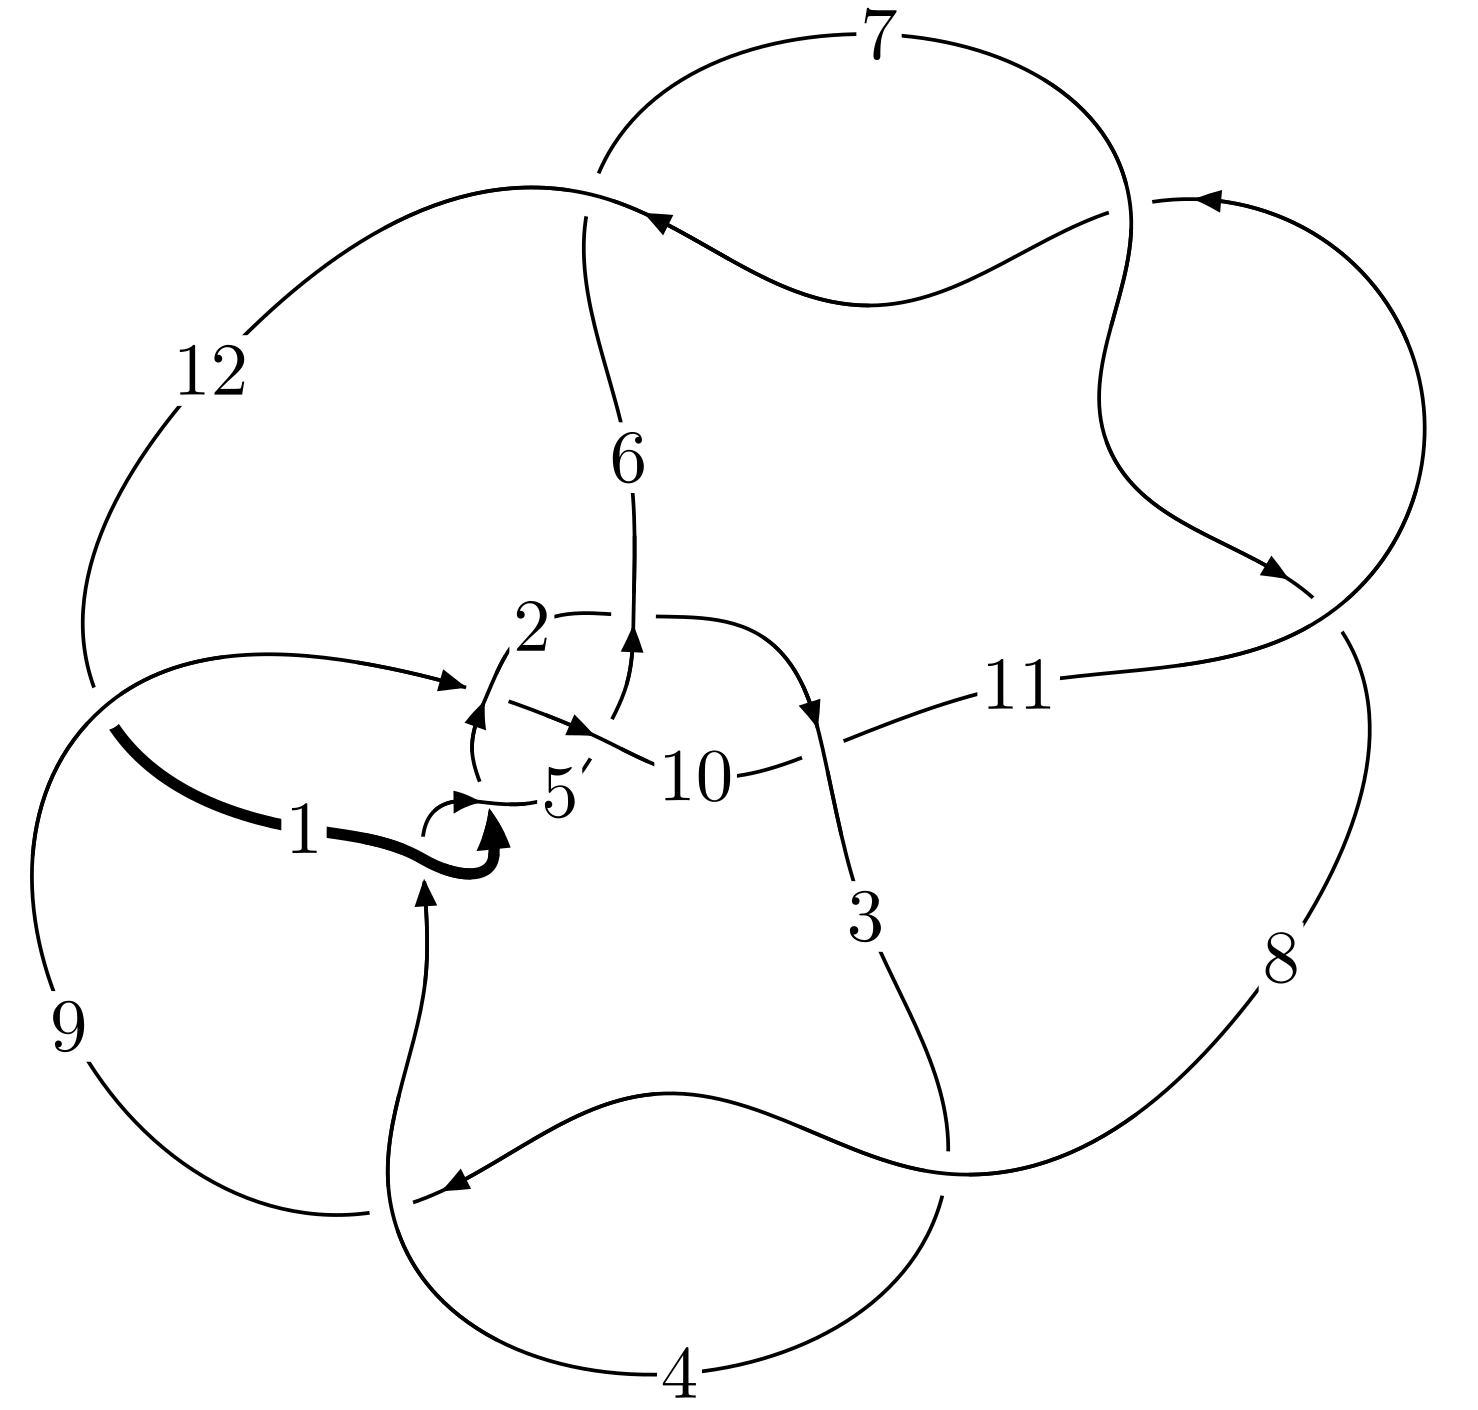
\includegraphics[width=112pt]{../../../GIT/diagram.site/Diagrams/png/2033_12a_1232.png}\\
\ \ \ A knot diagram\footnotemark}&
\allowdisplaybreaks
\textbf{Linearized knot diagam} \\
\cline{2-2}
 &
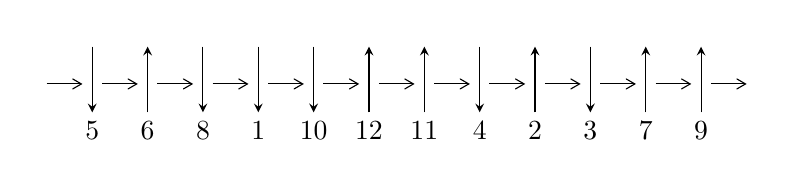
\begin{tikzpicture}[x=20pt, y=17pt]
	% nodes
	\node (C0) at (0, 0) {};
	\node (C1) at (1, 0) {};
	\node (C1U) at (1, +1) {};
	\node (C1D) at (1, -1) {5};

	\node (C2) at (2, 0) {};
	\node (C2U) at (2, +1) {};
	\node (C2D) at (2, -1) {6};

	\node (C3) at (3, 0) {};
	\node (C3U) at (3, +1) {};
	\node (C3D) at (3, -1) {8};

	\node (C4) at (4, 0) {};
	\node (C4U) at (4, +1) {};
	\node (C4D) at (4, -1) {1};

	\node (C5) at (5, 0) {};
	\node (C5U) at (5, +1) {};
	\node (C5D) at (5, -1) {10};

	\node (C6) at (6, 0) {};
	\node (C6U) at (6, +1) {};
	\node (C6D) at (6, -1) {12};

	\node (C7) at (7, 0) {};
	\node (C7U) at (7, +1) {};
	\node (C7D) at (7, -1) {11};

	\node (C8) at (8, 0) {};
	\node (C8U) at (8, +1) {};
	\node (C8D) at (8, -1) {4};

	\node (C9) at (9, 0) {};
	\node (C9U) at (9, +1) {};
	\node (C9D) at (9, -1) {2};

	\node (C10) at (10, 0) {};
	\node (C10U) at (10, +1) {};
	\node (C10D) at (10, -1) {3};

	\node (C11) at (11, 0) {};
	\node (C11U) at (11, +1) {};
	\node (C11D) at (11, -1) {7};

	\node (C12) at (12, 0) {};
	\node (C12U) at (12, +1) {};
	\node (C12D) at (12, -1) {9};
	\node (C13) at (13, 0) {};

	% arrows
	\draw[->,>={angle 60}]
	(C0) edge (C1) (C1) edge (C2) (C2) edge (C3) (C3) edge (C4) (C4) edge (C5) (C5) edge (C6) (C6) edge (C7) (C7) edge (C8) (C8) edge (C9) (C9) edge (C10) (C10) edge (C11) (C11) edge (C12) (C12) edge (C13) ;	\draw[->,>=stealth]
	(C1U) edge (C1D) (C2D) edge (C2U) (C3U) edge (C3D) (C4U) edge (C4D) (C5U) edge (C5D) (C6D) edge (C6U) (C7D) edge (C7U) (C8U) edge (C8D) (C9D) edge (C9U) (C10U) edge (C10D) (C11D) edge (C11U) (C12D) edge (C12U) ;
	\end{tikzpicture} \\
\hhline{~~} \\& 
\textbf{Solving Sequence} \\ \cline{2-2} 
 &
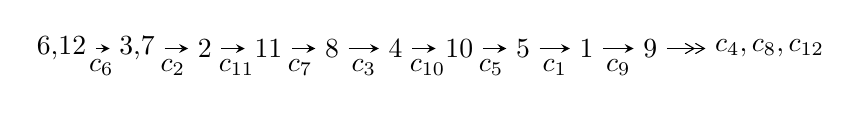
\begin{tikzpicture}[x=23pt, y=7pt]
	% node
	\node (A0) at (-1/8, 0) {6,12};
	\node (A1) at (17/16, 0) {3,7};
	\node (A2) at (17/8, 0) {2};
	\node (A3) at (25/8, 0) {11};
	\node (A4) at (33/8, 0) {8};
	\node (A5) at (41/8, 0) {4};
	\node (A6) at (49/8, 0) {10};
	\node (A7) at (57/8, 0) {5};
	\node (A8) at (65/8, 0) {1};
	\node (A9) at (73/8, 0) {9};
	\node (C1) at (1/2, -1) {$c_{6}$};
	\node (C2) at (13/8, -1) {$c_{2}$};
	\node (C3) at (21/8, -1) {$c_{11}$};
	\node (C4) at (29/8, -1) {$c_{7}$};
	\node (C5) at (37/8, -1) {$c_{3}$};
	\node (C6) at (45/8, -1) {$c_{10}$};
	\node (C7) at (53/8, -1) {$c_{5}$};
	\node (C8) at (61/8, -1) {$c_{1}$};
	\node (C9) at (69/8, -1) {$c_{9}$};
	\node (A10) at (11, 0) {$c_{4},c_{8},c_{12}$};

	% edge
	\draw[->,>=stealth]	
	(A0) edge (A1) (A1) edge (A2) (A2) edge (A3) (A3) edge (A4) (A4) edge (A5) (A5) edge (A6) (A6) edge (A7) (A7) edge (A8) (A8) edge (A9) ;
	\draw[->>,>={angle 60}]	
	(A9) edge (A10);
\end{tikzpicture} \\ 

\end{tabular} \\

\footnotetext{
The image of knot diagram is generated by the software ``\textbf{Draw programme}" developed by Andrew Bartholomew(\url{http://www.layer8.co.uk/maths/draw/index.htm\#Running-draw}), where we modified some parts for our purpose(\url{https://github.com/CATsTAILs/LinksPainter}).
}\phantom \\ \newline 
\centering \textbf{Ideals for irreducible components\footnotemark of $X_{\text{par}}$} 
 
\begin{align*}
I^u_{1}&=\langle 
2.89325\times10^{306} u^{118}+3.49433\times10^{305} u^{117}+\cdots+7.17437\times10^{304} b-1.65991\times10^{307},\\
\phantom{I^u_{1}}&\phantom{= \langle  }5.97626\times10^{306} u^{118}+1.91269\times10^{306} u^{117}+\cdots+7.17437\times10^{304} a-2.59098\times10^{307},\\
\phantom{I^u_{1}}&\phantom{= \langle  }u^{119}+60 u^{117}+\cdots-29 u+1\rangle \\
I^u_{2}&=\langle 
1182833 u^{25}-1697022 u^{24}+\cdots+999751 b+1307016,\\
\phantom{I^u_{2}}&\phantom{= \langle  }699334 u^{25}-115279 u^{24}+\cdots+999751 a-710366,\;u^{26}- u^{25}+\cdots-2 u-1\rangle \\
\\
\end{align*}
\raggedright * 2 irreducible components of $\dim_{\mathbb{C}}=0$, with total 145 representations.\\
\footnotetext{All coefficients of polynomials are rational numbers. But the coefficients are sometimes approximated in decimal forms when there is not enough margin.}
\newpage
\renewcommand{\arraystretch}{1}
\centering \section*{I. $I^u_{1}= \langle 2.89\times10^{306} u^{118}+3.49\times10^{305} u^{117}+\cdots+7.17\times10^{304} b-1.66\times10^{307},\;5.98\times10^{306} u^{118}+1.91\times10^{306} u^{117}+\cdots+7.17\times10^{304} a-2.59\times10^{307},\;u^{119}+60 u^{117}+\cdots-29 u+1 \rangle$}
\flushleft \textbf{(i) Arc colorings}\\
\begin{tabular}{m{7pt} m{180pt} m{7pt} m{180pt} }
\flushright $a_{6}=$&$\begin{pmatrix}1\\0\end{pmatrix}$ \\
\flushright $a_{12}=$&$\begin{pmatrix}0\\u\end{pmatrix}$ \\
\flushright $a_{3}=$&$\begin{pmatrix}-83.3000 u^{118}-26.6600 u^{117}+\cdots-8081.92 u+361.144\\-40.3276 u^{118}-4.87057 u^{117}+\cdots-5447.13 u+231.367\end{pmatrix}$ \\
\flushright $a_{7}=$&$\begin{pmatrix}1\\- u^2\end{pmatrix}$ \\
\flushright $a_{2}=$&$\begin{pmatrix}-42.9724 u^{118}-21.7895 u^{117}+\cdots-2634.78 u+129.777\\-40.3276 u^{118}-4.87057 u^{117}+\cdots-5447.13 u+231.367\end{pmatrix}$ \\
\flushright $a_{11}=$&$\begin{pmatrix}- u\\u^3+u\end{pmatrix}$ \\
\flushright $a_{8}=$&$\begin{pmatrix}u^2+1\\- u^4-2 u^2\end{pmatrix}$ \\
\flushright $a_{4}=$&$\begin{pmatrix}-22.7499 u^{118}-16.3719 u^{117}+\cdots-809.600 u+57.3880\\-43.6735 u^{118}-5.12507 u^{117}+\cdots-5969.86 u+253.459\end{pmatrix}$ \\
\flushright $a_{10}=$&$\begin{pmatrix}251.367 u^{118}+57.0280 u^{117}+\cdots+24863.9 u-978.564\\11.0833 u^{118}+1.80824 u^{117}+\cdots+1574.85 u-65.1638\end{pmatrix}$ \\
\flushright $a_{5}=$&$\begin{pmatrix}-244.071 u^{118}-67.7073 u^{117}+\cdots-21891.1 u+883.760\\-33.8994 u^{118}-5.61169 u^{117}+\cdots-4226.54 u+172.113\end{pmatrix}$ \\
\flushright $a_{1}=$&$\begin{pmatrix}233.063 u^{118}+65.0804 u^{117}+\cdots+20760.4 u-837.137\\37.1734 u^{118}+5.78030 u^{117}+\cdots+4678.97 u-191.478\end{pmatrix}$ \\
\flushright $a_{9}=$&$\begin{pmatrix}197.686 u^{118}+37.0655 u^{117}+\cdots+23253.8 u-939.916\\-16.1524 u^{118}-1.71445 u^{117}+\cdots-2346.84 u+105.264\end{pmatrix}$\\&\end{tabular}
\flushleft \textbf{(ii) Obstruction class $= -1$}\\~\\
\flushleft \textbf{(iii) Cusp Shapes $= 181.233 u^{118}+10.2983 u^{117}+\cdots+32671.8 u-1505.80$}\\~\\
\newpage\renewcommand{\arraystretch}{1}
\flushleft \textbf{(iv) u-Polynomials at the component}\newline \\
\begin{tabular}{m{50pt}|m{274pt}}
Crossings & \hspace{64pt}u-Polynomials at each crossing \\
\hline $$\begin{aligned}c_{1},c_{4}\end{aligned}$$&$\begin{aligned}
&u^{119}-3 u^{118}+\cdots+27 u+1
\end{aligned}$\\
\hline $$\begin{aligned}c_{2}\end{aligned}$$&$\begin{aligned}
&u^{119}-2 u^{118}+\cdots+6606 u+599
\end{aligned}$\\
\hline $$\begin{aligned}c_{3},c_{8}\end{aligned}$$&$\begin{aligned}
&u^{119}-2 u^{118}+\cdots+4224 u+256
\end{aligned}$\\
\hline $$\begin{aligned}c_{5}\end{aligned}$$&$\begin{aligned}
&u^{119}-2 u^{118}+\cdots+35541 u-6657
\end{aligned}$\\
\hline $$\begin{aligned}c_{6},c_{7},c_{11}\end{aligned}$$&$\begin{aligned}
&u^{119}+60 u^{117}+\cdots-29 u-1
\end{aligned}$\\
\hline $$\begin{aligned}c_{9}\end{aligned}$$&$\begin{aligned}
&u^{119}-2 u^{118}+\cdots+336 u+32
\end{aligned}$\\
\hline $$\begin{aligned}c_{10}\end{aligned}$$&$\begin{aligned}
&u^{119}-3 u^{118}+\cdots-8551161 u-339289
\end{aligned}$\\
\hline $$\begin{aligned}c_{12}\end{aligned}$$&$\begin{aligned}
&u^{119}+30 u^{117}+\cdots+3540492 u-1096431
\end{aligned}$\\
\hline
\end{tabular}\\~\\
\newpage\renewcommand{\arraystretch}{1}
\flushleft \textbf{(v) Riley Polynomials at the component}\newline \\
\begin{tabular}{m{50pt}|m{274pt}}
Crossings & \hspace{64pt}Riley Polynomials at each crossing \\
\hline $$\begin{aligned}c_{1},c_{4}\end{aligned}$$&$\begin{aligned}
&y^{119}-97 y^{118}+\cdots-215 y-1
\end{aligned}$\\
\hline $$\begin{aligned}c_{2}\end{aligned}$$&$\begin{aligned}
&y^{119}+12 y^{118}+\cdots-5057068 y-358801
\end{aligned}$\\
\hline $$\begin{aligned}c_{3},c_{8}\end{aligned}$$&$\begin{aligned}
&y^{119}-92 y^{118}+\cdots+14237696 y-65536
\end{aligned}$\\
\hline $$\begin{aligned}c_{5}\end{aligned}$$&$\begin{aligned}
&y^{119}-30 y^{118}+\cdots+3233514855 y-44315649
\end{aligned}$\\
\hline $$\begin{aligned}c_{6},c_{7},c_{11}\end{aligned}$$&$\begin{aligned}
&y^{119}+120 y^{118}+\cdots+91 y-1
\end{aligned}$\\
\hline $$\begin{aligned}c_{9}\end{aligned}$$&$\begin{aligned}
&y^{119}+32 y^{118}+\cdots-17664 y-1024
\end{aligned}$\\
\hline $$\begin{aligned}c_{10}\end{aligned}$$&$\begin{aligned}
&y^{119}-59 y^{118}+\cdots+46085256831797 y-115117025521
\end{aligned}$\\
\hline $$\begin{aligned}c_{12}\end{aligned}$$&$\begin{aligned}
&y^{119}+60 y^{118}+\cdots-19447210016610 y-1202160937761
\end{aligned}$\\
\hline
\end{tabular}\\~\\
\newpage\flushleft \textbf{(vi) Complex Volumes and Cusp Shapes}
$$\begin{array}{c|c|c}  
\text{Solutions to }I^u_{1}& \I (\text{vol} + \sqrt{-1}CS) & \text{Cusp shape}\\
 \hline 
\begin{aligned}
u &= -0.591023 + 0.831885 I \\
a &= \phantom{-}0.047144 + 0.336442 I \\
b &= -1.01813 - 1.09825 I\end{aligned}
 & -8.32691 - 5.97177 I & \phantom{-0.000000 } 0 \\ \hline\begin{aligned}
u &= -0.591023 - 0.831885 I \\
a &= \phantom{-}0.047144 - 0.336442 I \\
b &= -1.01813 + 1.09825 I\end{aligned}
 & -8.32691 + 5.97177 I & \phantom{-0.000000 } 0 \\ \hline\begin{aligned}
u &= \phantom{-}0.929575 + 0.429042 I \\
a &= \phantom{-}0.278050 - 0.303252 I \\
b &= -0.021658 - 0.248649 I\end{aligned}
 & -2.48998 + 0.81239 I & \phantom{-0.000000 } 0 \\ \hline\begin{aligned}
u &= \phantom{-}0.929575 - 0.429042 I \\
a &= \phantom{-}0.278050 + 0.303252 I \\
b &= -0.021658 + 0.248649 I\end{aligned}
 & -2.48998 - 0.81239 I & \phantom{-0.000000 } 0 \\ \hline\begin{aligned}
u &= -0.878703 + 0.541598 I \\
a &= \phantom{-}0.859638 + 0.663822 I \\
b &= -1.10195 + 1.05798 I\end{aligned}
 & -8.0032 - 13.9385 I & \phantom{-0.000000 } 0 \\ \hline\begin{aligned}
u &= -0.878703 - 0.541598 I \\
a &= \phantom{-}0.859638 - 0.663822 I \\
b &= -1.10195 - 1.05798 I\end{aligned}
 & -8.0032 + 13.9385 I & \phantom{-0.000000 } 0 \\ \hline\begin{aligned}
u &= -1.040530 + 0.281693 I \\
a &= \phantom{-}1.41699 + 0.17592 I \\
b &= -1.71346 + 0.91872 I\end{aligned}
 & -6.32387 + 0.55372 I & \phantom{-0.000000 } 0 \\ \hline\begin{aligned}
u &= -1.040530 - 0.281693 I \\
a &= \phantom{-}1.41699 - 0.17592 I \\
b &= -1.71346 - 0.91872 I\end{aligned}
 & -6.32387 - 0.55372 I & \phantom{-0.000000 } 0 \\ \hline\begin{aligned}
u &= \phantom{-}0.759955 + 0.784286 I \\
a &= \phantom{-}0.189923 + 0.583218 I \\
b &= \phantom{-}0.454075 + 0.072889 I\end{aligned}
 & -3.85449 + 4.96150 I & \phantom{-0.000000 } 0 \\ \hline\begin{aligned}
u &= \phantom{-}0.759955 - 0.784286 I \\
a &= \phantom{-}0.189923 - 0.583218 I \\
b &= \phantom{-}0.454075 - 0.072889 I\end{aligned}
 & -3.85449 - 4.96150 I & \phantom{-0.000000 } 0\\
 \hline 
 \end{array}$$\newpage$$\begin{array}{c|c|c}  
\text{Solutions to }I^u_{1}& \I (\text{vol} + \sqrt{-1}CS) & \text{Cusp shape}\\
 \hline 
\begin{aligned}
u &= -0.938198 + 0.565758 I \\
a &= -0.840420 - 0.416741 I \\
b &= \phantom{-}1.01130 - 1.18706 I\end{aligned}
 & -2.40547 - 7.97541 I & \phantom{-0.000000 } 0 \\ \hline\begin{aligned}
u &= -0.938198 - 0.565758 I \\
a &= -0.840420 + 0.416741 I \\
b &= \phantom{-}1.01130 + 1.18706 I\end{aligned}
 & -2.40547 + 7.97541 I & \phantom{-0.000000 } 0 \\ \hline\begin{aligned}
u &= \phantom{-}0.254868 + 0.867341 I \\
a &= -0.662773 - 0.261601 I \\
b &= -0.910213 + 0.623377 I\end{aligned}
 & \phantom{-}0.531296 - 1.118430 I & \phantom{-0.000000 } 0 \\ \hline\begin{aligned}
u &= \phantom{-}0.254868 - 0.867341 I \\
a &= -0.662773 + 0.261601 I \\
b &= -0.910213 - 0.623377 I\end{aligned}
 & \phantom{-}0.531296 + 1.118430 I & \phantom{-0.000000 } 0 \\ \hline\begin{aligned}
u &= -0.860183 + 0.680504 I \\
a &= -0.271297 + 0.232206 I \\
b &= -0.816520 - 1.081920 I\end{aligned}
 & -8.36465 + 8.14127 I & \phantom{-0.000000 } 0 \\ \hline\begin{aligned}
u &= -0.860183 - 0.680504 I \\
a &= -0.271297 - 0.232206 I \\
b &= -0.816520 + 1.081920 I\end{aligned}
 & -8.36465 - 8.14127 I & \phantom{-0.000000 } 0 \\ \hline\begin{aligned}
u &= \phantom{-}0.514362 + 1.042610 I \\
a &= \phantom{-}0.762760 + 0.248966 I \\
b &= \phantom{-}0.376032 - 0.566846 I\end{aligned}
 & -3.91604 + 4.65546 I & \phantom{-0.000000 } 0 \\ \hline\begin{aligned}
u &= \phantom{-}0.514362 - 1.042610 I \\
a &= \phantom{-}0.762760 - 0.248966 I \\
b &= \phantom{-}0.376032 + 0.566846 I\end{aligned}
 & -3.91604 - 4.65546 I & \phantom{-0.000000 } 0 \\ \hline\begin{aligned}
u &= -0.831661\phantom{ +0.000000I} \\
a &= -0.447104\phantom{ +0.000000I} \\
b &= \phantom{-}0.545531\phantom{ +0.000000I}\end{aligned}
 & \phantom{-}1.62981\phantom{ +0.000000I} & \phantom{-0.000000 } 0 \\ \hline\begin{aligned}
u &= \phantom{-}0.617128 + 0.557033 I \\
a &= -0.373648 + 1.101410 I \\
b &= \phantom{-}0.645942 + 0.638367 I\end{aligned}
 & -3.70214 + 3.85902 I & \phantom{-0.000000 } 0\\
 \hline 
 \end{array}$$\newpage$$\begin{array}{c|c|c}  
\text{Solutions to }I^u_{1}& \I (\text{vol} + \sqrt{-1}CS) & \text{Cusp shape}\\
 \hline 
\begin{aligned}
u &= \phantom{-}0.617128 - 0.557033 I \\
a &= -0.373648 - 1.101410 I \\
b &= \phantom{-}0.645942 - 0.638367 I\end{aligned}
 & -3.70214 - 3.85902 I & \phantom{-0.000000 } 0 \\ \hline\begin{aligned}
u &= \phantom{-}0.662911 + 0.486859 I \\
a &= \phantom{-}0.651270 - 0.915729 I \\
b &= -0.467298 - 0.951647 I\end{aligned}
 & -8.36947 + 5.21328 I & \phantom{-0.000000 } 0 \\ \hline\begin{aligned}
u &= \phantom{-}0.662911 - 0.486859 I \\
a &= \phantom{-}0.651270 + 0.915729 I \\
b &= -0.467298 + 0.951647 I\end{aligned}
 & -8.36947 - 5.21328 I & \phantom{-0.000000 } 0 \\ \hline\begin{aligned}
u &= \phantom{-}0.026248 + 1.183780 I \\
a &= \phantom{-}1.42598 + 0.72188 I \\
b &= -0.136361 - 0.409768 I\end{aligned}
 & -7.35451 - 5.52858 I & \phantom{-0.000000 } 0 \\ \hline\begin{aligned}
u &= \phantom{-}0.026248 - 1.183780 I \\
a &= \phantom{-}1.42598 - 0.72188 I \\
b &= -0.136361 + 0.409768 I\end{aligned}
 & -7.35451 + 5.52858 I & \phantom{-0.000000 } 0 \\ \hline\begin{aligned}
u &= \phantom{-}0.503026 + 0.641170 I \\
a &= \phantom{-}0.00117 - 1.61623 I \\
b &= -0.931842 - 0.533648 I\end{aligned}
 & -6.66685 + 3.36692 I & \phantom{-0.000000 } 0 \\ \hline\begin{aligned}
u &= \phantom{-}0.503026 - 0.641170 I \\
a &= \phantom{-}0.00117 + 1.61623 I \\
b &= -0.931842 + 0.533648 I\end{aligned}
 & -6.66685 - 3.36692 I & \phantom{-0.000000 } 0 \\ \hline\begin{aligned}
u &= -0.481513 + 1.086760 I \\
a &= -0.030737 - 0.313607 I \\
b &= \phantom{-}0.601979 - 0.325771 I\end{aligned}
 & -1.54373 - 4.64229 I & \phantom{-0.000000 } 0 \\ \hline\begin{aligned}
u &= -0.481513 - 1.086760 I \\
a &= -0.030737 + 0.313607 I \\
b &= \phantom{-}0.601979 + 0.325771 I\end{aligned}
 & -1.54373 + 4.64229 I & \phantom{-0.000000 } 0 \\ \hline\begin{aligned}
u &= -0.910620 + 0.774844 I \\
a &= \phantom{-}0.347935 - 0.275750 I \\
b &= \phantom{-}0.65714 + 1.37806 I\end{aligned}
 & -2.92800 + 1.74319 I & \phantom{-0.000000 } 0\\
 \hline 
 \end{array}$$\newpage$$\begin{array}{c|c|c}  
\text{Solutions to }I^u_{1}& \I (\text{vol} + \sqrt{-1}CS) & \text{Cusp shape}\\
 \hline 
\begin{aligned}
u &= -0.910620 - 0.774844 I \\
a &= \phantom{-}0.347935 + 0.275750 I \\
b &= \phantom{-}0.65714 - 1.37806 I\end{aligned}
 & -2.92800 - 1.74319 I & \phantom{-0.000000 } 0 \\ \hline\begin{aligned}
u &= \phantom{-}0.134503 + 0.759809 I \\
a &= -1.048930 - 0.154825 I \\
b &= \phantom{-}0.334044 + 0.899616 I\end{aligned}
 & -1.51344 - 1.60308 I & \phantom{-0.000000 } 0 \\ \hline\begin{aligned}
u &= \phantom{-}0.134503 - 0.759809 I \\
a &= -1.048930 + 0.154825 I \\
b &= \phantom{-}0.334044 - 0.899616 I\end{aligned}
 & -1.51344 + 1.60308 I & \phantom{-0.000000 } 0 \\ \hline\begin{aligned}
u &= -0.651277 + 0.410844 I \\
a &= \phantom{-}0.121534 + 0.601571 I \\
b &= -0.672685 + 0.188026 I\end{aligned}
 & \phantom{-}0.31785 - 2.06901 I & \phantom{-0.000000 } 0 \\ \hline\begin{aligned}
u &= -0.651277 - 0.410844 I \\
a &= \phantom{-}0.121534 - 0.601571 I \\
b &= -0.672685 - 0.188026 I\end{aligned}
 & \phantom{-}0.31785 + 2.06901 I & \phantom{-0.000000 } 0 \\ \hline\begin{aligned}
u &= \phantom{-}0.637309 + 0.424902 I \\
a &= -0.773608 + 0.372483 I \\
b &= -0.298804 + 0.749974 I\end{aligned}
 & -8.28201 - 0.92421 I & \phantom{-0.000000 } 0 \\ \hline\begin{aligned}
u &= \phantom{-}0.637309 - 0.424902 I \\
a &= -0.773608 - 0.372483 I \\
b &= -0.298804 - 0.749974 I\end{aligned}
 & -8.28201 + 0.92421 I & \phantom{-0.000000 } 0 \\ \hline\begin{aligned}
u &= \phantom{-}0.368271 + 0.658976 I \\
a &= \phantom{-}0.943588 + 0.048235 I \\
b &= \phantom{-}0.861584 - 0.736406 I\end{aligned}
 & -2.98116 - 5.40207 I & \phantom{-0.000000 } 0 \\ \hline\begin{aligned}
u &= \phantom{-}0.368271 - 0.658976 I \\
a &= \phantom{-}0.943588 - 0.048235 I \\
b &= \phantom{-}0.861584 + 0.736406 I\end{aligned}
 & -2.98116 + 5.40207 I & \phantom{-0.000000 } 0 \\ \hline\begin{aligned}
u &= -0.241125 + 1.258970 I \\
a &= -0.564327 - 0.615697 I \\
b &= \phantom{-}0.744666 - 0.214876 I\end{aligned}
 & -1.98462 - 3.32511 I & \phantom{-0.000000 } 0\\
 \hline 
 \end{array}$$\newpage$$\begin{array}{c|c|c}  
\text{Solutions to }I^u_{1}& \I (\text{vol} + \sqrt{-1}CS) & \text{Cusp shape}\\
 \hline 
\begin{aligned}
u &= -0.241125 - 1.258970 I \\
a &= -0.564327 + 0.615697 I \\
b &= \phantom{-}0.744666 + 0.214876 I\end{aligned}
 & -1.98462 + 3.32511 I & \phantom{-0.000000 } 0 \\ \hline\begin{aligned}
u &= \phantom{-}0.605698 + 0.366147 I \\
a &= -0.861264 + 0.880738 I \\
b &= \phantom{-}1.04506 + 0.98985 I\end{aligned}
 & -2.03512 + 8.97085 I & \phantom{-0.000000 } 0 \\ \hline\begin{aligned}
u &= \phantom{-}0.605698 - 0.366147 I \\
a &= -0.861264 - 0.880738 I \\
b &= \phantom{-}1.04506 - 0.98985 I\end{aligned}
 & -2.03512 - 8.97085 I & \phantom{-0.000000 } 0 \\ \hline\begin{aligned}
u &= -0.166818 + 1.294900 I \\
a &= \phantom{-}1.151150 + 0.222395 I \\
b &= -0.712514 + 0.315471 I\end{aligned}
 & -6.06217 - 4.53983 I & \phantom{-0.000000 } 0 \\ \hline\begin{aligned}
u &= -0.166818 - 1.294900 I \\
a &= \phantom{-}1.151150 - 0.222395 I \\
b &= -0.712514 - 0.315471 I\end{aligned}
 & -6.06217 + 4.53983 I & \phantom{-0.000000 } 0 \\ \hline\begin{aligned}
u &= -0.120884 + 1.327580 I \\
a &= -0.35980 - 1.40170 I \\
b &= \phantom{-}0.217292 - 0.220142 I\end{aligned}
 & -2.23327 - 2.51869 I & \phantom{-0.000000 } 0 \\ \hline\begin{aligned}
u &= -0.120884 - 1.327580 I \\
a &= -0.35980 + 1.40170 I \\
b &= \phantom{-}0.217292 + 0.220142 I\end{aligned}
 & -2.23327 + 2.51869 I & \phantom{-0.000000 } 0 \\ \hline\begin{aligned}
u &= \phantom{-}0.571093 + 0.340077 I \\
a &= \phantom{-}1.053790 - 0.767289 I \\
b &= -1.10538 - 0.88887 I\end{aligned}
 & \phantom{-}1.94608 + 4.33794 I & \phantom{-0.000000 } 0 \\ \hline\begin{aligned}
u &= \phantom{-}0.571093 - 0.340077 I \\
a &= \phantom{-}1.053790 + 0.767289 I \\
b &= -1.10538 + 0.88887 I\end{aligned}
 & \phantom{-}1.94608 - 4.33794 I & \phantom{-0.000000 } 0 \\ \hline\begin{aligned}
u &= -0.057455 + 1.348540 I \\
a &= \phantom{-}0.02930 + 1.77735 I \\
b &= \phantom{-}0.214941 + 0.235472 I\end{aligned}
 & -5.78869 + 0.62760 I & \phantom{-0.000000 } 0\\
 \hline 
 \end{array}$$\newpage$$\begin{array}{c|c|c}  
\text{Solutions to }I^u_{1}& \I (\text{vol} + \sqrt{-1}CS) & \text{Cusp shape}\\
 \hline 
\begin{aligned}
u &= -0.057455 - 1.348540 I \\
a &= \phantom{-}0.02930 - 1.77735 I \\
b &= \phantom{-}0.214941 - 0.235472 I\end{aligned}
 & -5.78869 - 0.62760 I & \phantom{-0.000000 } 0 \\ \hline\begin{aligned}
u &= -0.636266 + 0.018138 I \\
a &= -1.194210 - 0.458376 I \\
b &= \phantom{-}0.565733 + 0.080646 I\end{aligned}
 & \phantom{-}1.85506 + 0.08588 I & \phantom{-0.000000 } 0 \\ \hline\begin{aligned}
u &= -0.636266 - 0.018138 I \\
a &= -1.194210 + 0.458376 I \\
b &= \phantom{-}0.565733 - 0.080646 I\end{aligned}
 & \phantom{-}1.85506 - 0.08588 I & \phantom{-0.000000 } 0 \\ \hline\begin{aligned}
u &= -0.021921 + 1.412250 I \\
a &= -0.69650 - 3.75238 I \\
b &= -0.72366 - 3.51990 I\end{aligned}
 & -8.25856 + 0.30428 I & \phantom{-0.000000 } 0 \\ \hline\begin{aligned}
u &= -0.021921 - 1.412250 I \\
a &= -0.69650 + 3.75238 I \\
b &= -0.72366 + 3.51990 I\end{aligned}
 & -8.25856 - 0.30428 I & \phantom{-0.000000 } 0 \\ \hline\begin{aligned}
u &= -0.258157 + 0.517897 I \\
a &= -0.314448 + 0.579498 I \\
b &= -0.540503 + 0.493848 I\end{aligned}
 & \phantom{-}0.062363 - 1.273300 I & \phantom{-0.000000 } 0 \\ \hline\begin{aligned}
u &= -0.258157 - 0.517897 I \\
a &= -0.314448 - 0.579498 I \\
b &= -0.540503 - 0.493848 I\end{aligned}
 & \phantom{-}0.062363 + 1.273300 I & \phantom{-0.000000 } 0 \\ \hline\begin{aligned}
u &= \phantom{-}0.04031 + 1.42700 I \\
a &= \phantom{-}0.929315 + 0.791738 I \\
b &= \phantom{-}1.68565 + 0.62103 I\end{aligned}
 & -7.25607 - 0.01809 I & \phantom{-0.000000 } 0 \\ \hline\begin{aligned}
u &= \phantom{-}0.04031 - 1.42700 I \\
a &= \phantom{-}0.929315 - 0.791738 I \\
b &= \phantom{-}1.68565 - 0.62103 I\end{aligned}
 & -7.25607 + 0.01809 I & \phantom{-0.000000 } 0 \\ \hline\begin{aligned}
u &= \phantom{-}0.05079 + 1.43415 I \\
a &= \phantom{-}0.184273 - 0.284520 I \\
b &= -1.217520 - 0.235372 I\end{aligned}
 & -4.69275 + 3.59509 I & \phantom{-0.000000 } 0\\
 \hline 
 \end{array}$$\newpage$$\begin{array}{c|c|c}  
\text{Solutions to }I^u_{1}& \I (\text{vol} + \sqrt{-1}CS) & \text{Cusp shape}\\
 \hline 
\begin{aligned}
u &= \phantom{-}0.05079 - 1.43415 I \\
a &= \phantom{-}0.184273 + 0.284520 I \\
b &= -1.217520 + 0.235372 I\end{aligned}
 & -4.69275 - 3.59509 I & \phantom{-0.000000 } 0 \\ \hline\begin{aligned}
u &= \phantom{-}0.01595 + 1.44083 I \\
a &= \phantom{-}1.61897 - 1.36902 I \\
b &= \phantom{-}1.96434 - 1.03754 I\end{aligned}
 & -7.70307 + 0.43252 I & \phantom{-0.000000 } 0 \\ \hline\begin{aligned}
u &= \phantom{-}0.01595 - 1.44083 I \\
a &= \phantom{-}1.61897 + 1.36902 I \\
b &= \phantom{-}1.96434 + 1.03754 I\end{aligned}
 & -7.70307 - 0.43252 I & \phantom{-0.000000 } 0 \\ \hline\begin{aligned}
u &= \phantom{-}0.05041 + 1.44086 I \\
a &= -0.689485 - 0.103391 I \\
b &= \phantom{-}1.084470 + 0.136647 I\end{aligned}
 & -9.32231 + 7.31791 I & \phantom{-0.000000 } 0 \\ \hline\begin{aligned}
u &= \phantom{-}0.05041 - 1.44086 I \\
a &= -0.689485 + 0.103391 I \\
b &= \phantom{-}1.084470 - 0.136647 I\end{aligned}
 & -9.32231 - 7.31791 I & \phantom{-0.000000 } 0 \\ \hline\begin{aligned}
u &= \phantom{-}0.557225\phantom{ +0.000000I} \\
a &= \phantom{-}0.0193469\phantom{ +0.000000I} \\
b &= -1.31410\phantom{ +0.000000I}\end{aligned}
 & -4.86433\phantom{ +0.000000I} & \phantom{-}2.86400\phantom{ +0.000000I} \\ \hline\begin{aligned}
u &= -0.22188 + 1.42957 I \\
a &= -0.118268 + 1.125370 I \\
b &= -0.625169 + 0.517732 I\end{aligned}
 & -5.55217 - 5.25684 I & \phantom{-0.000000 } 0 \\ \hline\begin{aligned}
u &= -0.22188 - 1.42957 I \\
a &= -0.118268 - 1.125370 I \\
b &= -0.625169 - 0.517732 I\end{aligned}
 & -5.55217 + 5.25684 I & \phantom{-0.000000 } 0 \\ \hline\begin{aligned}
u &= \phantom{-}0.04350 + 1.45713 I \\
a &= -0.63772 + 1.50879 I \\
b &= -1.082230 + 0.548323 I\end{aligned}
 & -13.38820 + 0.81730 I & \phantom{-0.000000 } 0 \\ \hline\begin{aligned}
u &= \phantom{-}0.04350 - 1.45713 I \\
a &= -0.63772 - 1.50879 I \\
b &= -1.082230 - 0.548323 I\end{aligned}
 & -13.38820 - 0.81730 I & \phantom{-0.000000 } 0\\
 \hline 
 \end{array}$$\newpage$$\begin{array}{c|c|c}  
\text{Solutions to }I^u_{1}& \I (\text{vol} + \sqrt{-1}CS) & \text{Cusp shape}\\
 \hline 
\begin{aligned}
u &= \phantom{-}0.528301\phantom{ +0.000000I} \\
a &= \phantom{-}0.390274\phantom{ +0.000000I} \\
b &= \phantom{-}0.830129\phantom{ +0.000000I}\end{aligned}
 & -2.57760\phantom{ +0.000000I} & -9.17750\phantom{ +0.000000I} \\ \hline\begin{aligned}
u &= -0.03806 + 1.47195 I \\
a &= -0.45788 + 1.74878 I \\
b &= -0.500311 + 1.271440 I\end{aligned}
 & -6.29840 - 2.04801 I & \phantom{-0.000000 } 0 \\ \hline\begin{aligned}
u &= -0.03806 - 1.47195 I \\
a &= -0.45788 - 1.74878 I \\
b &= -0.500311 - 1.271440 I\end{aligned}
 & -6.29840 + 2.04801 I & \phantom{-0.000000 } 0 \\ \hline\begin{aligned}
u &= \phantom{-}0.16944 + 1.46677 I \\
a &= \phantom{-}0.29323 + 1.73137 I \\
b &= \phantom{-}1.41944 + 0.86687 I\end{aligned}
 & -8.31951 + 2.00416 I & \phantom{-0.000000 } 0 \\ \hline\begin{aligned}
u &= \phantom{-}0.16944 - 1.46677 I \\
a &= \phantom{-}0.29323 - 1.73137 I \\
b &= \phantom{-}1.41944 - 0.86687 I\end{aligned}
 & -8.31951 - 2.00416 I & \phantom{-0.000000 } 0 \\ \hline\begin{aligned}
u &= \phantom{-}0.17918 + 1.46604 I \\
a &= -0.36401 - 1.98590 I \\
b &= -1.30593 - 1.21078 I\end{aligned}
 & -3.97415 + 7.00684 I & \phantom{-0.000000 } 0 \\ \hline\begin{aligned}
u &= \phantom{-}0.17918 - 1.46604 I \\
a &= -0.36401 + 1.98590 I \\
b &= -1.30593 + 1.21078 I\end{aligned}
 & -3.97415 - 7.00684 I & \phantom{-0.000000 } 0 \\ \hline\begin{aligned}
u &= \phantom{-}0.19485 + 1.46412 I \\
a &= \phantom{-}0.27613 + 2.10943 I \\
b &= \phantom{-}1.16791 + 1.31696 I\end{aligned}
 & -7.9944 + 11.8379 I & \phantom{-0.000000 } 0 \\ \hline\begin{aligned}
u &= \phantom{-}0.19485 - 1.46412 I \\
a &= \phantom{-}0.27613 - 2.10943 I \\
b &= \phantom{-}1.16791 - 1.31696 I\end{aligned}
 & -7.9944 - 11.8379 I & \phantom{-0.000000 } 0 \\ \hline\begin{aligned}
u &= \phantom{-}0.28158 + 1.46280 I \\
a &= -0.745256 + 1.108810 I \\
b &= \phantom{-}0.116123 + 0.770788 I\end{aligned}
 & -14.2158 + 2.5074 I & \phantom{-0.000000 } 0\\
 \hline 
 \end{array}$$\newpage$$\begin{array}{c|c|c}  
\text{Solutions to }I^u_{1}& \I (\text{vol} + \sqrt{-1}CS) & \text{Cusp shape}\\
 \hline 
\begin{aligned}
u &= \phantom{-}0.28158 - 1.46280 I \\
a &= -0.745256 - 1.108810 I \\
b &= \phantom{-}0.116123 - 0.770788 I\end{aligned}
 & -14.2158 - 2.5074 I & \phantom{-0.000000 } 0 \\ \hline\begin{aligned}
u &= \phantom{-}0.415476 + 0.247825 I \\
a &= -1.013440 - 0.324156 I \\
b &= \phantom{-}0.953135 + 0.672474 I\end{aligned}
 & -1.89504 - 1.11164 I & \phantom{-}1.40333 + 1.47744 I \\ \hline\begin{aligned}
u &= \phantom{-}0.415476 - 0.247825 I \\
a &= -1.013440 + 0.324156 I \\
b &= \phantom{-}0.953135 - 0.672474 I\end{aligned}
 & -1.89504 + 1.11164 I & \phantom{-}1.40333 - 1.47744 I \\ \hline\begin{aligned}
u &= \phantom{-}0.23466 + 1.50340 I \\
a &= \phantom{-}0.27500 - 1.83384 I \\
b &= -0.545370 - 1.149990 I\end{aligned}
 & -14.8499 + 8.5093 I & \phantom{-0.000000 } 0 \\ \hline\begin{aligned}
u &= \phantom{-}0.23466 - 1.50340 I \\
a &= \phantom{-}0.27500 + 1.83384 I \\
b &= -0.545370 + 1.149990 I\end{aligned}
 & -14.8499 - 8.5093 I & \phantom{-0.000000 } 0 \\ \hline\begin{aligned}
u &= -0.474600 + 0.055730 I \\
a &= \phantom{-}2.06366 - 1.96246 I \\
b &= -0.297864 + 0.331525 I\end{aligned}
 & -1.89244 - 2.16716 I & \phantom{-}2.30593 + 6.36380 I \\ \hline\begin{aligned}
u &= -0.474600 - 0.055730 I \\
a &= \phantom{-}2.06366 + 1.96246 I \\
b &= -0.297864 - 0.331525 I\end{aligned}
 & -1.89244 + 2.16716 I & \phantom{-}2.30593 - 6.36380 I \\ \hline\begin{aligned}
u &= \phantom{-}0.407149 + 0.233846 I \\
a &= -2.38663 + 0.94353 I \\
b &= \phantom{-}1.029560 + 0.497453 I\end{aligned}
 & -2.62653 - 0.30445 I & -6.95283 - 7.49302 I \\ \hline\begin{aligned}
u &= \phantom{-}0.407149 - 0.233846 I \\
a &= -2.38663 - 0.94353 I \\
b &= \phantom{-}1.029560 - 0.497453 I\end{aligned}
 & -2.62653 + 0.30445 I & -6.95283 + 7.49302 I \\ \hline\begin{aligned}
u &= -0.01331 + 1.53266 I \\
a &= \phantom{-}0.70207 - 1.39377 I \\
b &= \phantom{-}0.683472 - 0.957463 I\end{aligned}
 & -10.39010 - 4.77458 I & \phantom{-0.000000 } 0\\
 \hline 
 \end{array}$$\newpage$$\begin{array}{c|c|c}  
\text{Solutions to }I^u_{1}& \I (\text{vol} + \sqrt{-1}CS) & \text{Cusp shape}\\
 \hline 
\begin{aligned}
u &= -0.01331 - 1.53266 I \\
a &= \phantom{-}0.70207 + 1.39377 I \\
b &= \phantom{-}0.683472 + 0.957463 I\end{aligned}
 & -10.39010 + 4.77458 I & \phantom{-0.000000 } 0 \\ \hline\begin{aligned}
u &= \phantom{-}0.22101 + 1.52748 I \\
a &= \phantom{-}0.01541 + 1.66790 I \\
b &= \phantom{-}0.700855 + 0.919045 I\end{aligned}
 & -10.52310 + 6.99423 I & \phantom{-0.000000 } 0 \\ \hline\begin{aligned}
u &= \phantom{-}0.22101 - 1.52748 I \\
a &= \phantom{-}0.01541 - 1.66790 I \\
b &= \phantom{-}0.700855 - 0.919045 I\end{aligned}
 & -10.52310 - 6.99423 I & \phantom{-0.000000 } 0 \\ \hline\begin{aligned}
u &= \phantom{-}0.18883 + 1.55710 I \\
a &= -0.33907 - 1.67862 I \\
b &= -0.862950 - 0.758452 I\end{aligned}
 & -13.9494 + 6.0462 I & \phantom{-0.000000 } 0 \\ \hline\begin{aligned}
u &= \phantom{-}0.18883 - 1.55710 I \\
a &= -0.33907 + 1.67862 I \\
b &= -0.862950 + 0.758452 I\end{aligned}
 & -13.9494 - 6.0462 I & \phantom{-0.000000 } 0 \\ \hline\begin{aligned}
u &= \phantom{-}0.31565 + 1.54001 I \\
a &= \phantom{-}0.231980 - 0.980002 I \\
b &= -0.340835 - 0.610925 I\end{aligned}
 & -8.96711 + 5.30293 I & \phantom{-0.000000 } 0 \\ \hline\begin{aligned}
u &= \phantom{-}0.31565 - 1.54001 I \\
a &= \phantom{-}0.231980 + 0.980002 I \\
b &= -0.340835 + 0.610925 I\end{aligned}
 & -8.96711 - 5.30293 I & \phantom{-0.000000 } 0 \\ \hline\begin{aligned}
u &= -0.30992 + 1.55607 I \\
a &= \phantom{-}0.02307 + 1.74012 I \\
b &= -1.31776 + 1.13652 I\end{aligned}
 & -14.8309 - 18.2934 I & \phantom{-0.000000 } 0 \\ \hline\begin{aligned}
u &= -0.30992 - 1.55607 I \\
a &= \phantom{-}0.02307 - 1.74012 I \\
b &= -1.31776 - 1.13652 I\end{aligned}
 & -14.8309 + 18.2934 I & \phantom{-0.000000 } 0 \\ \hline\begin{aligned}
u &= -0.16255 + 1.58538 I \\
a &= -0.87747 - 1.33760 I \\
b &= -0.92126 - 1.73717 I\end{aligned}
 & -16.2984 - 8.6510 I & \phantom{-0.000000 } 0\\
 \hline 
 \end{array}$$\newpage$$\begin{array}{c|c|c}  
\text{Solutions to }I^u_{1}& \I (\text{vol} + \sqrt{-1}CS) & \text{Cusp shape}\\
 \hline 
\begin{aligned}
u &= -0.16255 - 1.58538 I \\
a &= -0.87747 + 1.33760 I \\
b &= -0.92126 + 1.73717 I\end{aligned}
 & -16.2984 + 8.6510 I & \phantom{-0.000000 } 0 \\ \hline\begin{aligned}
u &= -0.31935 + 1.57309 I \\
a &= -0.03812 - 1.63961 I \\
b &= \phantom{-}1.33515 - 1.22468 I\end{aligned}
 & -9.3806 - 12.5591 I & \phantom{-0.000000 } 0 \\ \hline\begin{aligned}
u &= -0.31935 - 1.57309 I \\
a &= -0.03812 + 1.63961 I \\
b &= \phantom{-}1.33515 + 1.22468 I\end{aligned}
 & -9.3806 + 12.5591 I & \phantom{-0.000000 } 0 \\ \hline\begin{aligned}
u &= \phantom{-}0.26564 + 1.60378 I \\
a &= \phantom{-}0.212361 + 1.045510 I \\
b &= \phantom{-}0.584964 + 0.515464 I\end{aligned}
 & -11.6412 + 8.8735 I & \phantom{-0.000000 } 0 \\ \hline\begin{aligned}
u &= \phantom{-}0.26564 - 1.60378 I \\
a &= \phantom{-}0.212361 - 1.045510 I \\
b &= \phantom{-}0.584964 - 0.515464 I\end{aligned}
 & -11.6412 - 8.8735 I & \phantom{-0.000000 } 0 \\ \hline\begin{aligned}
u &= -0.41085 + 1.58525 I \\
a &= \phantom{-}0.12577 + 1.53275 I \\
b &= -1.84219 + 1.27507 I\end{aligned}
 & -12.44770 - 4.97409 I & \phantom{-0.000000 } 0 \\ \hline\begin{aligned}
u &= -0.41085 - 1.58525 I \\
a &= \phantom{-}0.12577 - 1.53275 I \\
b &= -1.84219 - 1.27507 I\end{aligned}
 & -12.44770 + 4.97409 I & \phantom{-0.000000 } 0 \\ \hline\begin{aligned}
u &= -0.22405 + 1.63859 I \\
a &= -0.612798 - 0.975425 I \\
b &= -0.49612 - 1.37066 I\end{aligned}
 & -16.2469 + 4.0696 I & \phantom{-0.000000 } 0 \\ \hline\begin{aligned}
u &= -0.22405 - 1.63859 I \\
a &= -0.612798 + 0.975425 I \\
b &= -0.49612 + 1.37066 I\end{aligned}
 & -16.2469 - 4.0696 I & \phantom{-0.000000 } 0 \\ \hline\begin{aligned}
u &= -0.17895 + 1.64890 I \\
a &= \phantom{-}0.599878 + 1.274540 I \\
b &= \phantom{-}0.50996 + 1.83509 I\end{aligned}
 & -11.42610 - 2.22065 I & \phantom{-0.000000 } 0\\
 \hline 
 \end{array}$$\newpage$$\begin{array}{c|c|c}  
\text{Solutions to }I^u_{1}& \I (\text{vol} + \sqrt{-1}CS) & \text{Cusp shape}\\
 \hline 
\begin{aligned}
u &= -0.17895 - 1.64890 I \\
a &= \phantom{-}0.599878 - 1.274540 I \\
b &= \phantom{-}0.50996 - 1.83509 I\end{aligned}
 & -11.42610 + 2.22065 I & \phantom{-0.000000 } 0 \\ \hline\begin{aligned}
u &= -0.163226 + 0.233600 I \\
a &= \phantom{-}0.647394 - 0.912052 I \\
b &= \phantom{-}0.23639 - 1.44563 I\end{aligned}
 & -3.02302 + 0.92759 I & -16.4734 + 13.4457 I \\ \hline\begin{aligned}
u &= -0.163226 - 0.233600 I \\
a &= \phantom{-}0.647394 + 0.912052 I \\
b &= \phantom{-}0.23639 + 1.44563 I\end{aligned}
 & -3.02302 - 0.92759 I & -16.4734 - 13.4457 I \\ \hline\begin{aligned}
u &= \phantom{-}0.223493 + 0.145601 I \\
a &= \phantom{-}3.91291 + 2.79472 I \\
b &= -0.731943 - 0.378521 I\end{aligned}
 & \phantom{-}0.63117 + 2.73482 I & \phantom{-}4.06228 - 7.56761 I \\ \hline\begin{aligned}
u &= \phantom{-}0.223493 - 0.145601 I \\
a &= \phantom{-}3.91291 - 2.79472 I \\
b &= -0.731943 + 0.378521 I\end{aligned}
 & \phantom{-}0.63117 - 2.73482 I & \phantom{-}4.06228 + 7.56761 I \\ \hline\begin{aligned}
u &= \phantom{-}0.186898 + 0.120104 I \\
a &= -5.16636 - 6.62078 I \\
b &= \phantom{-}0.688517 + 0.325209 I\end{aligned}
 & -3.96488 + 6.53995 I & \phantom{-}4.08042 - 8.20161 I \\ \hline\begin{aligned}
u &= \phantom{-}0.186898 - 0.120104 I \\
a &= -5.16636 + 6.62078 I \\
b &= \phantom{-}0.688517 - 0.325209 I\end{aligned}
 & -3.96488 - 6.53995 I & \phantom{-}4.08042 + 8.20161 I \\ \hline\begin{aligned}
u &= \phantom{-}0.193994\phantom{ +0.000000I} \\
a &= -7.22223\phantom{ +0.000000I} \\
b &= -0.820442\phantom{ +0.000000I}\end{aligned}
 & -8.08181\phantom{ +0.000000I} & -11.4190\phantom{ +0.000000I} \\ \hline\begin{aligned}
u &= \phantom{-}0.155376\phantom{ +0.000000I} \\
a &= \phantom{-}2.35334\phantom{ +0.000000I} \\
b &= \phantom{-}1.49630\phantom{ +0.000000I}\end{aligned}
 & -2.45224\phantom{ +0.000000I} & -30.3120\phantom{ +0.000000I}\\
 \hline 
 \end{array}$$\newpage\newpage\renewcommand{\arraystretch}{1}
\centering \section*{II. $I^u_{2}= \langle 1.18\times10^{6} u^{25}-1.70\times10^{6} u^{24}+\cdots+1.00\times10^{6} b+1.31\times10^{6},\;6.99\times10^{5} u^{25}-1.15\times10^{5} u^{24}+\cdots+1.00\times10^{6} a-7.10\times10^{5},\;u^{26}- u^{25}+\cdots-2 u-1 \rangle$}
\flushleft \textbf{(i) Arc colorings}\\
\begin{tabular}{m{7pt} m{180pt} m{7pt} m{180pt} }
\flushright $a_{6}=$&$\begin{pmatrix}1\\0\end{pmatrix}$ \\
\flushright $a_{12}=$&$\begin{pmatrix}0\\u\end{pmatrix}$ \\
\flushright $a_{3}=$&$\begin{pmatrix}-0.699508 u^{25}+0.115308 u^{24}+\cdots+2.44780 u+0.710543\\-1.18313 u^{25}+1.69744 u^{24}+\cdots+0.755925 u-1.30734\end{pmatrix}$ \\
\flushright $a_{7}=$&$\begin{pmatrix}1\\- u^2\end{pmatrix}$ \\
\flushright $a_{2}=$&$\begin{pmatrix}0.483619 u^{25}-1.58214 u^{24}+\cdots+1.69188 u+2.01788\\-1.18313 u^{25}+1.69744 u^{24}+\cdots+0.755925 u-1.30734\end{pmatrix}$ \\
\flushright $a_{11}=$&$\begin{pmatrix}- u\\u^3+u\end{pmatrix}$ \\
\flushright $a_{8}=$&$\begin{pmatrix}u^2+1\\- u^4-2 u^2\end{pmatrix}$ \\
\flushright $a_{4}=$&$\begin{pmatrix}-1.34719 u^{25}+1.12802 u^{24}+\cdots+2.92028 u+0.855845\\-0.872567 u^{25}+1.32808 u^{24}+\cdots+0.999658 u-1.43425\end{pmatrix}$ \\
\flushright $a_{10}=$&$\begin{pmatrix}-0.692340 u^{25}+1.51595 u^{24}+\cdots+4.24471 u+0.476967\\-0.312059 u^{25}+0.234258 u^{24}+\cdots+2.42780 u+0.800910\end{pmatrix}$ \\
\flushright $a_{5}=$&$\begin{pmatrix}-1.31393 u^{25}-0.798396 u^{24}+\cdots+10.0988 u+5.81141\\0.109095 u^{25}-0.0590167 u^{24}+\cdots+2.33029 u+0.702249\end{pmatrix}$ \\
\flushright $a_{1}=$&$\begin{pmatrix}-0.399081 u^{25}-1.97885 u^{24}+\cdots+8.79390 u+5.58117\\-0.310036 u^{25}+1.13491 u^{24}+\cdots+2.22230 u+0.190208\end{pmatrix}$ \\
\flushright $a_{9}=$&$\begin{pmatrix}-1.70690 u^{25}+1.91267 u^{24}+\cdots+4.45269 u-0.655580\\-0.312059 u^{25}+0.234258 u^{24}+\cdots+0.427805 u-0.199090\end{pmatrix}$\\&\end{tabular}
\flushleft \textbf{(ii) Obstruction class $= 1$}\\~\\
\flushleft \textbf{(iii) Cusp Shapes $= -\frac{5221017}{999751} u^{25}+\frac{13972069}{999751} u^{24}+\cdots-\frac{8621882}{999751} u-\frac{13731564}{999751}$}\\~\\
\newpage\renewcommand{\arraystretch}{1}
\flushleft \textbf{(iv) u-Polynomials at the component}\newline \\
\begin{tabular}{m{50pt}|m{274pt}}
Crossings & \hspace{64pt}u-Polynomials at each crossing \\
\hline $$\begin{aligned}c_{1}\end{aligned}$$&$\begin{aligned}
&u^{26}+4 u^{25}+\cdots+2 u-1
\end{aligned}$\\
\hline $$\begin{aligned}c_{2}\end{aligned}$$&$\begin{aligned}
&u^{26}-5 u^{25}+\cdots-3 u+1
\end{aligned}$\\
\hline $$\begin{aligned}c_{3}\end{aligned}$$&$\begin{aligned}
&u^{26}+u^{25}+\cdots+3 u+1
\end{aligned}$\\
\hline $$\begin{aligned}c_{4}\end{aligned}$$&$\begin{aligned}
&u^{26}-4 u^{25}+\cdots-2 u-1
\end{aligned}$\\
\hline $$\begin{aligned}c_{5}\end{aligned}$$&$\begin{aligned}
&u^{26}- u^{25}+\cdots-6 u^2+1
\end{aligned}$\\
\hline $$\begin{aligned}c_{6},c_{7}\end{aligned}$$&$\begin{aligned}
&u^{26}- u^{25}+\cdots-2 u-1
\end{aligned}$\\
\hline $$\begin{aligned}c_{8}\end{aligned}$$&$\begin{aligned}
&u^{26}- u^{25}+\cdots-3 u+1
\end{aligned}$\\
\hline $$\begin{aligned}c_{9}\end{aligned}$$&$\begin{aligned}
&u^{26}- u^{25}+\cdots+13 u^2-1
\end{aligned}$\\
\hline $$\begin{aligned}c_{10}\end{aligned}$$&$\begin{aligned}
&u^{26}+u^{24}+\cdots+2 u-1
\end{aligned}$\\
\hline $$\begin{aligned}c_{11}\end{aligned}$$&$\begin{aligned}
&u^{26}+u^{25}+\cdots+2 u-1
\end{aligned}$\\
\hline $$\begin{aligned}c_{12}\end{aligned}$$&$\begin{aligned}
&u^{26}+3 u^{25}+\cdots-3 u-1
\end{aligned}$\\
\hline
\end{tabular}\\~\\
\newpage\renewcommand{\arraystretch}{1}
\flushleft \textbf{(v) Riley Polynomials at the component}\newline \\
\begin{tabular}{m{50pt}|m{274pt}}
Crossings & \hspace{64pt}Riley Polynomials at each crossing \\
\hline $$\begin{aligned}c_{1},c_{4}\end{aligned}$$&$\begin{aligned}
&y^{26}-24 y^{25}+\cdots+14 y+1
\end{aligned}$\\
\hline $$\begin{aligned}c_{2}\end{aligned}$$&$\begin{aligned}
&y^{26}+5 y^{25}+\cdots-13 y+1
\end{aligned}$\\
\hline $$\begin{aligned}c_{3},c_{8}\end{aligned}$$&$\begin{aligned}
&y^{26}-7 y^{25}+\cdots-15 y+1
\end{aligned}$\\
\hline $$\begin{aligned}c_{5}\end{aligned}$$&$\begin{aligned}
&y^{26}- y^{25}+\cdots-12 y+1
\end{aligned}$\\
\hline $$\begin{aligned}c_{6},c_{7},c_{11}\end{aligned}$$&$\begin{aligned}
&y^{26}+25 y^{25}+\cdots+4 y+1
\end{aligned}$\\
\hline $$\begin{aligned}c_{9}\end{aligned}$$&$\begin{aligned}
&y^{26}+21 y^{25}+\cdots-26 y+1
\end{aligned}$\\
\hline $$\begin{aligned}c_{10}\end{aligned}$$&$\begin{aligned}
&y^{26}+2 y^{25}+\cdots-14 y+1
\end{aligned}$\\
\hline $$\begin{aligned}c_{12}\end{aligned}$$&$\begin{aligned}
&y^{26}+21 y^{25}+\cdots+65 y+1
\end{aligned}$\\
\hline
\end{tabular}\\~\\
\newpage\flushleft \textbf{(vi) Complex Volumes and Cusp Shapes}
$$\begin{array}{c|c|c}  
\text{Solutions to }I^u_{2}& \I (\text{vol} + \sqrt{-1}CS) & \text{Cusp shape}\\
 \hline 
\begin{aligned}
u &= \phantom{-}0.943663\phantom{ +0.000000I} \\
a &= -1.74187\phantom{ +0.000000I} \\
b &= \phantom{-}1.68335\phantom{ +0.000000I}\end{aligned}
 & -6.46795\phantom{ +0.000000I} & -10.5950\phantom{ +0.000000I} \\ \hline\begin{aligned}
u &= -0.262117 + 0.794880 I \\
a &= \phantom{-}1.206650 - 0.607794 I \\
b &= \phantom{-}0.636935 + 0.707784 I\end{aligned}
 & -0.29611 + 1.84881 I & -2.20099 - 5.13154 I \\ \hline\begin{aligned}
u &= -0.262117 - 0.794880 I \\
a &= \phantom{-}1.206650 + 0.607794 I \\
b &= \phantom{-}0.636935 - 0.707784 I\end{aligned}
 & -0.29611 - 1.84881 I & -2.20099 + 5.13154 I \\ \hline\begin{aligned}
u &= -0.427225 + 1.116590 I \\
a &= -0.552298 - 0.157514 I \\
b &= \phantom{-}0.432472 - 0.380122 I\end{aligned}
 & -2.00627 - 4.23987 I & -6.89686 + 3.43816 I \\ \hline\begin{aligned}
u &= -0.427225 - 1.116590 I \\
a &= -0.552298 + 0.157514 I \\
b &= \phantom{-}0.432472 + 0.380122 I\end{aligned}
 & -2.00627 + 4.23987 I & -6.89686 - 3.43816 I \\ \hline\begin{aligned}
u &= \phantom{-}0.736758 + 0.948318 I \\
a &= -0.111244 - 0.374605 I \\
b &= -0.430583 - 0.402133 I\end{aligned}
 & -4.15027 + 5.36590 I & -6.6302 - 15.0637 I \\ \hline\begin{aligned}
u &= \phantom{-}0.736758 - 0.948318 I \\
a &= -0.111244 + 0.374605 I \\
b &= -0.430583 + 0.402133 I\end{aligned}
 & -4.15027 - 5.36590 I & -6.6302 + 15.0637 I \\ \hline\begin{aligned}
u &= -0.798164\phantom{ +0.000000I} \\
a &= -0.720467\phantom{ +0.000000I} \\
b &= \phantom{-}0.451395\phantom{ +0.000000I}\end{aligned}
 & \phantom{-}1.31350\phantom{ +0.000000I} & -10.8780\phantom{ +0.000000I} \\ \hline\begin{aligned}
u &= -0.042885 + 1.222100 I \\
a &= \phantom{-}1.67307 + 0.59418 I \\
b &= -0.768144 + 0.390201 I\end{aligned}
 & -6.94373 - 6.67014 I & -4.82849 + 8.01150 I \\ \hline\begin{aligned}
u &= -0.042885 - 1.222100 I \\
a &= \phantom{-}1.67307 - 0.59418 I \\
b &= -0.768144 - 0.390201 I\end{aligned}
 & -6.94373 + 6.67014 I & -4.82849 - 8.01150 I\\
 \hline 
 \end{array}$$\newpage$$\begin{array}{c|c|c}  
\text{Solutions to }I^u_{2}& \I (\text{vol} + \sqrt{-1}CS) & \text{Cusp shape}\\
 \hline 
\begin{aligned}
u &= -0.178950 + 1.217590 I \\
a &= -0.818036 - 0.682512 I \\
b &= \phantom{-}0.772257 - 0.348218 I\end{aligned}
 & -1.91082 - 3.72292 I & -0.00835 + 12.45701 I \\ \hline\begin{aligned}
u &= -0.178950 - 1.217590 I \\
a &= -0.818036 + 0.682512 I \\
b &= \phantom{-}0.772257 + 0.348218 I\end{aligned}
 & -1.91082 + 3.72292 I & -0.00835 - 12.45701 I \\ \hline\begin{aligned}
u &= -0.189668 + 1.303550 I \\
a &= \phantom{-}0.008222 + 0.447989 I \\
b &= -0.934613 - 0.264739 I\end{aligned}
 & -6.27743 - 3.06539 I & -6.85778 + 2.47354 I \\ \hline\begin{aligned}
u &= -0.189668 - 1.303550 I \\
a &= \phantom{-}0.008222 - 0.447989 I \\
b &= -0.934613 + 0.264739 I\end{aligned}
 & -6.27743 + 3.06539 I & -6.85778 - 2.47354 I \\ \hline\begin{aligned}
u &= \phantom{-}0.582028 + 0.253462 I \\
a &= -0.0563762 + 0.0530277 I \\
b &= -0.945003 + 0.308953 I\end{aligned}
 & -2.17597 + 0.05862 I & \phantom{-}6.50604 - 2.22033 I \\ \hline\begin{aligned}
u &= \phantom{-}0.582028 - 0.253462 I \\
a &= -0.0563762 - 0.0530277 I \\
b &= -0.945003 - 0.308953 I\end{aligned}
 & -2.17597 - 0.05862 I & \phantom{-}6.50604 + 2.22033 I \\ \hline\begin{aligned}
u &= -0.01677 + 1.42907 I \\
a &= -1.36555 + 3.39416 I \\
b &= -1.54172 + 3.09921 I\end{aligned}
 & -8.10928 + 0.28326 I & -6.3171 + 26.2657 I \\ \hline\begin{aligned}
u &= -0.01677 - 1.42907 I \\
a &= -1.36555 - 3.39416 I \\
b &= -1.54172 - 3.09921 I\end{aligned}
 & -8.10928 - 0.28326 I & -6.3171 - 26.2657 I \\ \hline\begin{aligned}
u &= \phantom{-}0.028959 + 0.564258 I \\
a &= -2.77914 - 0.23608 I \\
b &= -0.634395 - 0.458952 I\end{aligned}
 & -4.55240 + 6.43356 I & -9.62563 - 6.14441 I \\ \hline\begin{aligned}
u &= \phantom{-}0.028959 - 0.564258 I \\
a &= -2.77914 + 0.23608 I \\
b &= -0.634395 + 0.458952 I\end{aligned}
 & -4.55240 - 6.43356 I & -9.62563 + 6.14441 I\\
 \hline 
 \end{array}$$\newpage$$\begin{array}{c|c|c}  
\text{Solutions to }I^u_{2}& \I (\text{vol} + \sqrt{-1}CS) & \text{Cusp shape}\\
 \hline 
\begin{aligned}
u &= \phantom{-}0.32913 + 1.53078 I \\
a &= -0.14874 + 1.51913 I \\
b &= \phantom{-}1.27469 + 0.92809 I\end{aligned}
 & -11.90070 + 4.72608 I & -4.74884 - 1.80377 I \\ \hline\begin{aligned}
u &= \phantom{-}0.32913 - 1.53078 I \\
a &= -0.14874 - 1.51913 I \\
b &= \phantom{-}1.27469 - 0.92809 I\end{aligned}
 & -11.90070 - 4.72608 I & -4.74884 + 1.80377 I \\ \hline\begin{aligned}
u &= \phantom{-}0.19195 + 1.56700 I \\
a &= -0.255553 - 1.353580 I \\
b &= -0.434170 - 0.756346 I\end{aligned}
 & -12.3990 + 8.2757 I & -10.18523 - 5.61464 I \\ \hline\begin{aligned}
u &= \phantom{-}0.19195 - 1.56700 I \\
a &= -0.255553 + 1.353580 I \\
b &= -0.434170 + 0.756346 I\end{aligned}
 & -12.3990 - 8.2757 I & -10.18523 + 5.61464 I \\ \hline\begin{aligned}
u &= -0.323951 + 0.201932 I \\
a &= \phantom{-}1.93017 + 0.80624 I \\
b &= -0.995098 + 0.915085 I\end{aligned}
 & -2.49812 + 0.92147 I & -6.47033 + 0.38560 I \\ \hline\begin{aligned}
u &= -0.323951 - 0.201932 I \\
a &= \phantom{-}1.93017 - 0.80624 I \\
b &= -0.995098 - 0.915085 I\end{aligned}
 & -2.49812 - 0.92147 I & -6.47033 - 0.38560 I\\
 \hline 
 \end{array}$$\newpage
\newpage\renewcommand{\arraystretch}{1}
\centering \section*{ III. u-Polynomials}
\begin{tabular}{m{50pt}|m{274pt}}
Crossings & \hspace{64pt}u-Polynomials at each crossing \\
\hline $$\begin{aligned}c_{1}\end{aligned}$$&$\begin{aligned}
&(u^{26}+4 u^{25}+\cdots+2 u-1)(u^{119}-3 u^{118}+\cdots+27 u+1)
\end{aligned}$\\
\hline $$\begin{aligned}c_{2}\end{aligned}$$&$\begin{aligned}
&(u^{26}-5 u^{25}+\cdots-3 u+1)(u^{119}-2 u^{118}+\cdots+6606 u+599)
\end{aligned}$\\
\hline $$\begin{aligned}c_{3}\end{aligned}$$&$\begin{aligned}
&(u^{26}+u^{25}+\cdots+3 u+1)(u^{119}-2 u^{118}+\cdots+4224 u+256)
\end{aligned}$\\
\hline $$\begin{aligned}c_{4}\end{aligned}$$&$\begin{aligned}
&(u^{26}-4 u^{25}+\cdots-2 u-1)(u^{119}-3 u^{118}+\cdots+27 u+1)
\end{aligned}$\\
\hline $$\begin{aligned}c_{5}\end{aligned}$$&$\begin{aligned}
&(u^{26}- u^{25}+\cdots-6 u^2+1)(u^{119}-2 u^{118}+\cdots+35541 u-6657)
\end{aligned}$\\
\hline $$\begin{aligned}c_{6},c_{7}\end{aligned}$$&$\begin{aligned}
&(u^{26}- u^{25}+\cdots-2 u-1)(u^{119}+60 u^{117}+\cdots-29 u-1)
\end{aligned}$\\
\hline $$\begin{aligned}c_{8}\end{aligned}$$&$\begin{aligned}
&(u^{26}- u^{25}+\cdots-3 u+1)(u^{119}-2 u^{118}+\cdots+4224 u+256)
\end{aligned}$\\
\hline $$\begin{aligned}c_{9}\end{aligned}$$&$\begin{aligned}
&(u^{26}- u^{25}+\cdots+13 u^2-1)(u^{119}-2 u^{118}+\cdots+336 u+32)
\end{aligned}$\\
\hline $$\begin{aligned}c_{10}\end{aligned}$$&$\begin{aligned}
&(u^{26}+u^{24}+\cdots+2 u-1)(u^{119}-3 u^{118}+\cdots-8551161 u-339289)
\end{aligned}$\\
\hline $$\begin{aligned}c_{11}\end{aligned}$$&$\begin{aligned}
&(u^{26}+u^{25}+\cdots+2 u-1)(u^{119}+60 u^{117}+\cdots-29 u-1)
\end{aligned}$\\
\hline $$\begin{aligned}c_{12}\end{aligned}$$&$\begin{aligned}
&(u^{26}+3 u^{25}+\cdots-3 u-1)\\
&\cdot(u^{119}+30 u^{117}+\cdots+3540492 u-1096431)
\end{aligned}$\\
\hline
\end{tabular}\newpage\renewcommand{\arraystretch}{1}
\centering \section*{ IV. Riley Polynomials}
\begin{tabular}{m{50pt}|m{274pt}}
Crossings & \hspace{64pt}Riley Polynomials at each crossing \\
\hline $$\begin{aligned}c_{1},c_{4}\end{aligned}$$&$\begin{aligned}
&(y^{26}-24 y^{25}+\cdots+14 y+1)(y^{119}-97 y^{118}+\cdots-215 y-1)
\end{aligned}$\\
\hline $$\begin{aligned}c_{2}\end{aligned}$$&$\begin{aligned}
&(y^{26}+5 y^{25}+\cdots-13 y+1)\\
&\cdot(y^{119}+12 y^{118}+\cdots-5057068 y-358801)
\end{aligned}$\\
\hline $$\begin{aligned}c_{3},c_{8}\end{aligned}$$&$\begin{aligned}
&(y^{26}-7 y^{25}+\cdots-15 y+1)\\
&\cdot(y^{119}-92 y^{118}+\cdots+14237696 y-65536)
\end{aligned}$\\
\hline $$\begin{aligned}c_{5}\end{aligned}$$&$\begin{aligned}
&(y^{26}- y^{25}+\cdots-12 y+1)\\
&\cdot(y^{119}-30 y^{118}+\cdots+3233514855 y-44315649)
\end{aligned}$\\
\hline $$\begin{aligned}c_{6},c_{7},c_{11}\end{aligned}$$&$\begin{aligned}
&(y^{26}+25 y^{25}+\cdots+4 y+1)(y^{119}+120 y^{118}+\cdots+91 y-1)
\end{aligned}$\\
\hline $$\begin{aligned}c_{9}\end{aligned}$$&$\begin{aligned}
&(y^{26}+21 y^{25}+\cdots-26 y+1)(y^{119}+32 y^{118}+\cdots-17664 y-1024)
\end{aligned}$\\
\hline $$\begin{aligned}c_{10}\end{aligned}$$&$\begin{aligned}
&(y^{26}+2 y^{25}+\cdots-14 y+1)\\
&\cdot(y^{119}-59 y^{118}+\cdots+46085256831797 y-115117025521)
\end{aligned}$\\
\hline $$\begin{aligned}c_{12}\end{aligned}$$&$\begin{aligned}
&(y^{26}+21 y^{25}+\cdots+65 y+1)\\
&\cdot(y^{119}+60 y^{118}+\cdots-19447210016610 y-1202160937761)
\end{aligned}$\\
\hline
\end{tabular}
\vskip 2pc
\end{document}